\section{Introduction}
\label{sec:introduction}

For a fixed graph $G$, consider
\begin{equation}
 m(G)=\min_{\sigma:E(G)\to\{\pm1\}}\rho(A_\sigma).
 \label{eq:fixed-minimum}
\end{equation}
Only the signs of the nonzero adjacency entries vary; the support, degrees,
and underlying cycles remain fixed.  Switching at vertices conjugates
$A_\sigma$ by a diagonal sign matrix, so its spectrum depends on the switching
class rather than on the individual edge labels.  Products of signs around
cycles are the surviving coordinates.  This passage from edge signs to cycle
data is already present in the balance and switching theory of Harary and
Zaslavsky \cite{Harary1953,Zaslavsky1982}, and it makes
\eqref{eq:fixed-minimum} a problem about organizing cycle signs on a fixed
support.

Spectral control by signings also has an important existence theory.  In a
two-lift, a signing governs the new eigenvalues; Bilu and Linial used this
relation in their work on discrepancy and spectral gaps, while Marcus,
Spielman, and Srivastava obtained sharp bipartite Ramanujan signings through
interlacing polynomials \cite{BiluLinial2006,MarcusSpielmanSrivastava2015}.
Those results ask whether some signing meets a universal benchmark.  The exact
fixed-graph problem asks more: what is the least radius for this particular
$G$, and which switching classes attain it?  This question belongs to the
broader spectral theory of signed graphs \cite{BelardoEtAl2018}; exact extrema
for restricted signed families show that fixing the underlying structure can
lead to rigid equality classes \cite{BrunettiStanic2022,GhorbaniMajidi2024}.

We study \eqref{eq:fixed-minimum} on
\[
 C_n(1,2),\qquad V=\mathbb Z/n\mathbb Z,\qquad
 i\sim j\iff i-j\equiv\pm1,\pm2\pmod n.
\]
The graph combines a one-dimensional cyclic backbone with an overlapping
triangle based at every vertex.  The first feature makes ordinary circulant
spectra accessible by Fourier analysis \cite{Davis1979}; the second localizes
the switching-invariant cycle data.  A periodic triangle-sign pattern preserves
translation by one cell even when one-site translation is lost.  Thus
$C_n(1,2)$ has both nontrivial local signed-cycle geometry and a tractable
matrix-valued Bloch symbol.  The gauge and flux language used below is the
finite signed-graph counterpart of the corresponding framework for unit-gain
and periodic magnetic graph operators
\cite{Reff2012,KorotyaevSaburova2017,KorotyaevSaburova2023}.

There is a natural reference level among periodic phases.  After the step-one
cycle is put in Hamilton gauge, the alternating triangle word
$\tau_i=(-1)^i$ has local square word $Q_i=\tau_i\tau_{i+1}=-1$ and squared
Bloch edge exactly $8$.  It is already chiral: an alternating diagonal sign
combined with half-period translation anticommutes with its fibers.  The
extremal question is therefore not whether chirality can occur at short
period, but whether a primitive periodic phase can push the squared edge
strictly below $8$.

The first such phase occurs at period eight.  In Hamilton-gauge triangle
coordinates and the associated local square coordinates it is
\begin{equation}
 \tau_*=(1,1,-1,1,-1,-1,1,-1),\qquad
 Q_*=(1,-1,-1,-1,1,-1,-1,-1).
 \label{eq:target-words}
\end{equation}
The two positive entries of $Q_*$ are antipodal; the second half of $\tau_*$
is the negative of the first.  Figure~\ref{fig:period8-cell} shows both
features on the cycle square.

\begin{figure}[t]
 \centering
 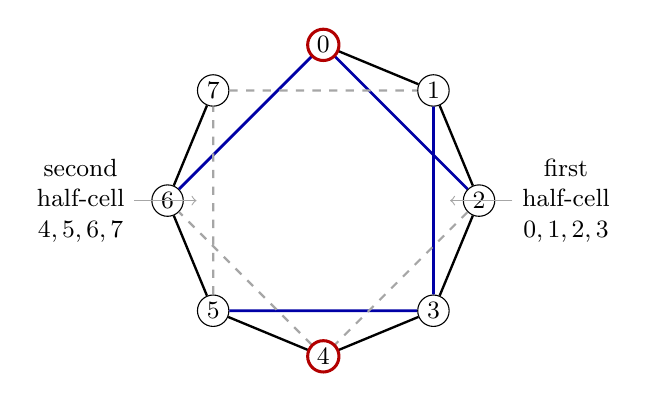
\begin{tikzpicture}[scale=0.92,
 vertex/.style={circle,draw,fill=white,inner sep=1.4pt,font=\small},
 defect/.style={circle,draw=red!70!black,line width=1.1pt,inner sep=4pt}]
 \node[vertex] (v0) at (90:2.15) {$0$};
 \node[vertex] (v1) at (45:2.15) {$1$};
 \node[vertex] (v2) at (0:2.15) {$2$};
 \node[vertex] (v3) at (-45:2.15) {$3$};
 \node[vertex] (v4) at (-90:2.15) {$4$};
 \node[vertex] (v5) at (-135:2.15) {$5$};
 \node[vertex] (v6) at (180:2.15) {$6$};
 \node[vertex] (v7) at (135:2.15) {$7$};
 \draw[line width=.85pt] (v0)--(v1)--(v2)--(v3)--(v4)--(v5)--(v6)--(v7)--cycle;
 \draw[blue!65!black,line width=1pt]
   (v0)--(v2) (v1)--(v3) (v3)--(v5) (v6)--(v0);
 \draw[gray!70,dashed,line width=.8pt]
   (v2)--(v4) (v4)--(v6) (v5)--(v7) (v7)--(v1);
 \node[defect] at (v0) {};
 \node[defect] at (v4) {};
 \node[font=\small,align=center] (hl) at (-3.35,0) {second\\half-cell\\$4,5,6,7$};
 \node[font=\small,align=center] (hr) at (3.35,0) {first\\half-cell\\$0,1,2,3$};
 \draw[->,gray!70] (hl.east)--(-1.75,0);
 \draw[->,gray!70] (hr.west)--(1.75,0);
\end{tikzpicture}

 \caption{The period-eight phase.  The black cycle is the locally positive
 step-one gauge.  Blue solid and gray dashed chords have positive and negative
 triangle flux, respectively.  The red vertices mark the two positive entries
 of $Q_*$.  Vertices $0,1,2,3$ form the first half-cell and vertices
 $4,5,6,7$ the second.}
 \label{fig:period8-cell}
\end{figure}

Let $A_{8L,+}^{*}$ be the finite signed adjacency matrix obtained by repeating
\eqref{eq:target-words} over $L$ cells with positive Hamilton holonomy, and set
\begin{equation}
 \etaedge=4+\sqrt{10+2\sqrt5}.
 \label{eq:eta}
\end{equation}
The first main result gives the radius of every finite member of this family.

\begin{theorem}
\label{thm:main-exact}
For every integer $L\geq1$,
\[
 \rho(A_{8L,+}^{*})^2=\etaedge.
\]
If $A_{8L}^{\mathrm{tw}}$ denotes the twisted signing defined in
\cref{sec:twisted}, then, for every $L\geq4$,
\[
 \rho(A_{8L,+}^{*})^2=\etaedge
   <\rho(A_{8L}^{\mathrm{tw}})^2.
\]
Consequently $m(C_{8L}(1,2))<\rho(A_{8L}^{\mathrm{tw}})$ for every $L\geq4$.
\end{theorem}

The equality holds on each finite ring, including $L=1$: it is not an
infinite-volume edge approached asymptotically.  The maximizing fiber is
present in every positive-holonomy phase grid.  The strict comparison begins
at $L=4$ and produces an infinite family of improvements over the twisted
benchmark.  These facts still leave the exact solvability unexplained.  Its
visible clue is the sign reversal $\tau_{i+4}=-\tau_i$.

That reversal is not peculiar to eight sites.  At an arbitrary even period it
is exactly the condition for a natural monomial half-cell symmetry, and the
same condition can be read without choosing a lift of the local square word.

\begin{theorem}
\label{thm:main-chiral}
Let $p=2m$ and let $\tau$ be a $2m$-periodic Hamilton-gauge word.  Within the
monomial class consisting of the alternating diagonal sign followed by
half-period translation, a normalized chiral involution exists on every Bloch
fiber if and only if
\[
 \tau_{i+m}=-\tau_i\qquad(i\in\mathbb Z).
\]
Equivalently, with $Q_i=\tau_i\tau_{i+1}$,
\[
 Q_{i+m}=Q_i\quad(i\in\mathbb Z),\qquad
 \prod_{j=0}^{m-1}Q_j=-1.
\]
Under these conditions the characteristic polynomial is even, and the squared
fiber problem reduces from dimension $2m$ to dimension $m$.
\end{theorem}

The equivalence converts an operator symmetry into switching-invariant local
graph data: half-periodicity of $Q$ and the sign accumulated over one
half-cell determine chirality.  Spectral symmetry for signed graph operators
and half-period chiral constructions occur in related settings
\cite{AtayHua2016,CedzichEtAl2021}; here the criterion is tied to the adjacency
operator on the cycle square.  Chirality alone does not lower the edge, as the
alternating period-two phase shows.  When, then, does the half-cell mechanism
first become spectrally effective?

\begin{theorem}
\label{thm:main-minimal}
Eight is the smallest primitive period of a legal Hamilton-gauge signing whose
squared Bloch edge is strictly below $8$.
\end{theorem}

Thus period eight is selected by the spectral threshold, not by the first
appearance of an anticommuting symmetry.  At the first effective period a
second question becomes unavoidable: is the low-edge phase isolated, or does
period eight contain several unrelated examples?

\begin{theorem}
\label{thm:main-rigidity}
Among legal period-eight $Q$-words, $Q_*$ is the unique dihedral orbit with
squared Bloch edge below $8$.  Its two $\tau$-lifts differ by a global sign and
have the same squared edge.  The all-negative $Q$-word has edge $8$, and every
other legal period-eight orbit has edge strictly above $8$.
\end{theorem}

The surviving orbit has two defects and places them as far apart as the cell
allows.  Low-order trace moments first penalize defect density and then
short-range clustering.  This explains the geometry of the short-period
classification without asserting a sufficiency theorem for arbitrary periods.
The same moments yield general necessary restrictions on defect density and
clustering, recorded after the period-eight proof.

A recent preprint proposed the twisted class as a global optimizer for every
even order \cite{Suvagiya2026}.  The strict inequality in
Theorem~\ref{thm:main-exact} disproves that proposal on every order $8L$ with
$L\geq4$.

Two ingredients drive the proofs.  A finite Bloch decomposition and the
half-cell involution reduce the period-eight spectrum to a centered quartic,
whose four bands and two finite holonomy sectors can be solved exactly.  A
local square identity and its first three trace moments reduce all shorter
periods and all period-eight competitors to a small set of configurations;
explicit integer and Rayleigh certificates close that set.  The first method
explains solvability, while the second explains first occurrence and rigidity.
